\documentclass{article}

\usepackage{amsthm}
\usepackage{amsmath}
\usepackage{cite}
\usepackage{listings}
\usepackage{multicol}
\usepackage{booktabs}
\usepackage{url}
\usepackage{xeCJK}
\usepackage{chngpage}
\usepackage{float}
\usepackage{graphicx}
\usepackage{setspace}
\usepackage[margin=1in]{geometry}
\usepackage[bottom]{footmisc}
\setCJKmainfont{IPAMincho}
\graphicspath{ {./images/} }
\onehalfspacing

\setlength{\parindent}{4em}
\setlength{\parskip}{1em}

\title{Transliterating English to Japanese Without Parallel Data}
\date{2019-04-22}
\author{Derick Anderson \\ anderson.de@husky.neu.edu
  \and Timothy Gillis \\ gillis.ti@husky.neu.edu }

\begin{document}

\pagenumbering{gobble}
\maketitle

\section*{Introduction}

We aim to learn to transliterate English to Japanese
without any parallel data.
That is to say,
given only monolingual corpora
and the tiniest insight about Japanese orthography
to learn how to represent English words in Japanese script.
Learning to transliterate with limited supervision has been well studied,
but there have been only limited attempts to learn without at least parallel data.
The key inspiration was the recent paper by
Conneau et al. \cite{Conneau2018WordTW}
in which word translations were learned with no parallel data
(or any other supervision).
Conneau et al. did not touch Japanese,
so we hope to first replicate their work on the Japanese-English language pair.
We then hope to discover an algorithm to learn to transliterate
using those (probably noisy) results as training data.

As big data becomes more readily available, the cost of manually labeling large
datasets emphasizes the need for unsupervised algorithms that perform as well if
not better than their supervised counterparts, and the cost of cleaning these
datasets highlights the need for algorithms to effectively handle noisy data as well.
Our project will touch upon both of these problems in the machine transliteration
sphere, specifically by first generating a Japanese-English dictionary in an
unsupervised way, then attempting to learn to transliterate from that noisy data.

Derick has a personal interest in Japanese, transliteration, and both together.
Timothy would like to gain experience in natural language processing and machine
translation.

\noindent
All of our code is available on GitHub
\footnote{https://github.com/dandersonw/ml-final-project}.

\section*{Background}

\subsection*{Transliteration}

Transliteration is representing words
in a script or orthographic style
other than that with which they were originally represented.
Between close scripts like the Old English alphabet and the modern English alphabet
this can be a mechanical character to character mapping:
e.g. ``þe olde'' to ``ye olde''.
Between distant scripts
like the English alphabet and Japanese katakana
the task becomes more difficult.
Translation includes transliteration as a subtask,
although the relationship between the two
depends on the language pair, intended audience, and other factors.

In the literature on machine transliteration there is a distinction
between generative transliteration and transliteration extraction.
Generative transliteration learns a function for transliterating;
transliteration extraction just identifies pairs of strings
to be added to a transliteration dictionary
\cite{Karimi:2011:MTS:1922649.1922654}.
In this paper we will be doing generative transliteration.

In translating into both English and Japanese
probably the most common use of transliteration
is representing foreign proper nouns.
Because proper nouns are an open and varied class
there has been a lot of work on unsupervised learning to transliterate them
(e.g. \cite{Tao2006UnsupervisedNE}),
maybe for use in machine translation (e.g. \cite{Durrani2014IntegratingAU})
or cross-language information retrieval (e.g. \cite{10.1007/978-3-642-40087-2_29}).
A limitation of our proposed approach
is that we will not pay any special attention to proper nouns,
which often have their own conventions for transliteration.

The use of transliteration most relevant to this project
is the borrowing of words from foreign languages.
Like proper nouns,
some words may not have equivalents in every language,
and rather than create a neologism from native material (e.g. as done in Icelandic)
a foreign word might be adopted and used.

The work most closely related to ours is that of Ravi and Knight
\cite{Ravi2009LearningPM}
who learn to back-transliterate from Japanese to English
without any parallel data.
Back-transliteration is the process of
transforming a katakana string that represents an English word
back into the English word it represents.
The Ravi and Knight work seems to be followed up some other work
like a paper by Levinboim et. al. \cite{Levinboim2015ModelIR}
which aims to improve the same basic approach.
The key difference between their approach and ours
is that theirs requires a well trained model of Japanese and English phonetics.
We may choose to utilize an English phonetic model,
but don't require either.
Furthermore,
they impose constraints and start with favorable intializations
based on prior knowledge about transliteration.
We will utilize the fact
that English words are translated into katakana,
but hope to not inject any other prior knowledge.
Learning to transliterate into katakana
without knowledge of their pronunciation
or much aid from prior knowledge should be a step forward.

\subsection*{The Japanese-English Language Pair}

In modern orthography
Japanese represents foreign words
by approximating the pronunciation of the foreign word
in a syllabary \footnote{In a syllabary each character represents a syllable,
although katakana has some exceptions by that definition.} called katakana.
Native Japanese words and loanwords from Chinese
\footnote{Words of Sinitic origin are so common in Japanese that they not considered
  foreign in the same sense as words from English.}
are usually represented in scripts besides katakana:
the hiragana syllabary and kanji
\footnote{``Kanji'' is the Japanese name for Chinese characters.}.
The approximation of pronunciation is really quite approximate;
because Japanese has a relatively limited phonetic inventory (range of sounds used)
not all English sounds can be represented.
In the face of the complicated correspondence
between English spelling and English pronunciation
(to say nothing of international English variants)
Japanese people sometimes transliterate based on the spelling of a word
rather than the pronunciation.
An ideal system,
therefore,
will probably need to consider both phonetics and spelling.

Japanese has taken many loan words from English.
These can be common nouns (bed, ベッド),
verbs (join, ジョイン),
adjectives (sexy, セクシー),
or even sentence pieces (let's!, レッツ!).
Many (most?) loan words
are used in the same ways as their English equivalents,
although the meaning of some has diverged.
Japanese has also taken loanwords from other languages
that are written in katakana,
some of which may conflict with English words.
An example is ナトリウム,
from the Latin natrium,
meaning sodium (consider the Na elemental abbreviation).
The hope is that clever matching of English words
will allow useful transcription pairs to be found.

\subsection*{Word Translation Without Parallel Data}

Last year, Conneau et al. proposed a state-of-the-art unsupervised method for machine
translation without using any parallel corpora, that works well for both distant
language pairs (e.g. English-Chinese, English-Japanese) and pairs with limited parallel
data (e.g. English-Esperanto), also outperforming supervised methods on some language
pairs. This is accomplished by aligning the monolingual word embedding spaces for each
language in the pair.

Supervised methods attempt to learn a linear mapping $W$ between the source and target
space such that $WX-Y$ is minimized, where $X$ and $Y$ are the source and target word
embedding pairs, respectively. Because they attempt to learn $W$ without cross-lingual 
supervision, they use a domain-adversarial approach, where a discriminator is trained
to discriminate between translated (i.e. generated) words and words actually from the
target domain, and $W$ is simultaneously trained to "fool" the discriminator by making
the generated words as similar to the target words as possible.

While the learned $W$ roughly aligns the two embedding spaces, Conneau et al add two
modifications to further align the spaces:

First, a refinement procedure is proposed where the $W$ trained via the
adversarial method is used to generate a synthetic parallel vocabulary, which is
then used to minimize $WX-Y$ in a supervised manner. More specifically, they use
the generated parallel vocabulary to apply the Procrustes solution (i.e.
min $\|WX-Y\|_2 = UV^T$, where $U\Sigma V^T = SVD(YX^T)$). This is repeated several
times, with the expectation being that the generated data improves each iteration.
This approach can also be "kickstarted" in a supervised manner by simply applying
the first iteration with a ground truth parallel vocabulary.

Second, they introduce a cross-domain similarity adaptation, cross-domain similarity
local scaling (CSLS), to mitigate the "hubness problem"
(i.e. in high dimensional spaces, some points tend to be nearest neighbors
to many other points). Specifically, they use the mean similarity of a source
embedding translation ($Wx_s$) to its target K nearest neighbors:
$$
r_T(Wx_s)=\frac{1}{K}\sum_{y_t \in \mathcal{N}_T(Wx_s)} \text{cos}(Wx_s, y_t)
$$
where $\mathcal{N}_T(Wx_s)$ is the K nearest neighbors of the source embedding
translation, and define the similarity metric as:
$$
\text{CSLS}(Wx_s,y_t)=2\text{cos}(Wx_s, y_t)-r_T(Wx_s)-r_S(y_t)
$$

\section*{Methods}

\subsection*{Unsupervised Word Translation}

\subsubsection*{Data}

We begin by downloading pre-trained monolingual word vectors for English, Japanese,
and all the other languages we plan to run experiments with \cite{bojanowski2017enriching}.
These are 300 dimensional word vectors trained on Wikipedia using fastText.
Although this project's overall goal is to learn transliteration for the specific
English-Japanese language pair, for this section we plan to more generally analyze
how well the approach described in Word Translation Without Parallel Data generalizes
to new language pairs, especially one of languages that are comparably as distant as
the English-Japanese pair.

Other than Japanese, we run experiments on the following languages paired with English:
Spanish, French, Chinese, Portuguese, Hebrew, Hindi, Thai, Korean, and Arabic. This
allows us to first reproduce their results on 3 language pairs, along with test their
method's generalization on 7 new language pairs of varying similarity.

\subsubsection*{Methodology}

As we are simply reproducing the results outlined in Word Translation Without Parallel
Data, we use the same training architecture and methodology. Firstly, only the 200k
most frequent words are loaded for training the mapping matrix $W$, and the 50k most
frequent for the discriminator. A two layered feed forward neural network is used
for the discriminator, with each hidden layer of size 2048, Leaky-ReLU activation
functions and a dropout rate of 0.1. The default training parameters for
both the discriminator and $W$ as described in the paper are a
batch size of 32, learning rate of 0.1, learning rate decay of 0.95, smoothing
coefficient of 0.2, epoch size of 250k and a learning rate shrink parameter of 0.5
(i.e. whenever the unsupervised validation criterion decreases after a training epoch
they divide the learning rate in half). We also apply the iterative refinement
procedure 8 times after the intial adversarial training, starting with the model with
the highest CSLS score. Optimization is done by stochastic gradient descent.
Since we find that their proposed validation
criterion does not correlate as well with word translation precision on new language
pairs, we change this shrink parameter to 0.75. Moreover, we normalize all embeddings
by subtracting the mean embedding.

\noindent
For the mapping matrix $W$'s update rule, an orthogonal constrant is imposed, where
$\beta=0.01$:
$$
W \leftarrow (1 + \beta)W - \beta(WW^T)W
$$

When generating the synthetic parallel data to be used for transliteration, we take
the aligned Japanese embedding space with the best word translation precision
at $\text{k}=1$ and generate proposed translations for the 50k most frequent
source words using CSLS. We choose the top 50k words since that is the largest
amount our computer can handle to perform CSLS on at the same time. While we could
run vanilla K nearest neighbors in "batches", this produces worse translations
since the hubness problem persists.

Although CSLS aims to reduce hubs, it does not completely solve the problem.
Therefore we first remove certain words from the target dictionary that qualitatively
show up as incorrect translations for many source words, these are mainly articles
and adverbs (e.g. and, to, the, moreover, at, nevertheless, then, likewise, etc.).
Then before transliteration, we filter out translated words that appear more than
20 times.

\subsubsection*{Evaluation}

The proposed validation metric CSLS is used with the 10k most frequent source words
for model selection (and when deciding to shrink the learning rate during training).
However for final evaluation, we simply use word translation precision at
$\text{k}=1$. This is to ensure the translations used for transliteration are as
accurate as possible.

\subsection*{Transliteration}

\subsubsection*{Data}

We use a few external sources of data.
Facebook Research provides a ground truth English-Japanese dictionary
of the same sort as is used for their evaluation of word translation,
available on their GitHub
\footnote{https://github.com/facebookresearch/MUSE}.
It contains about 14,000 translations of an English word to a katakana string.
We used this dictionary for evaluating the transliteration model
we learn on generated pairs.
Our thinking was that Facebook's ground truth dictionary
should be alike to the pairs we hope to generate from word translation
using their method.
We will refer to it as the ``MUSE'' data.
A concrete way in which that is true is that
there are no translation pairs with two English words,
unlike some other transliteration data available.
We use the dataset available here
\footnote{https://github.com/eob/english-japanese-transliteration}
because it is freely available,
of decent quality,
and referenced in the Google paper\cite{Rosca2016SequencetosequenceNN}
we use as a baseline.
We will refer to it as the ``eob'' data.
CMU makes available a large dataset of English words and their pronunciations
\footnote{http://www.speech.cs.cmu.edu/cgi-bin/cmudict},
which we will refer to as the ``CMU'' data.

\subsubsection*{Learning Transliteration: Basic}

Considering just the bird's eye view of the task
as transforming a sequence of characters to another sequence of characters,
our first thought was to use a sequence-to-sequence model
like the well known Google neural machine translation model
\cite{Wu2016GooglesNM}.
Not surprisingly,
some people at Google did try that \cite{Rosca2016SequencetosequenceNN}
and found that the results were highly competitive.
Since attentional sequence-to-sequence models \cite{Bahdanau2015NeuralMT}
are so well known,
we won't describe the basic architecture here.

Treating words as just sequences of characters
diverges from a lot of transliteration methods
in ignoring pronunciation.
The motivation for that
is that we don't have pronunciation information for translation-pairs
that we get out of the word translation half of the project.

All of the networks we use operate on a character basis.
Each script is a separate vocabulary;
the Japanese decoder can output only katakana characters
and the English encoder can read only English characters.
We operate on composed representations of Unicode characters:
e.g. ``ガ'' is represented by the atomic \texttt{U+X30AC KATAKANA LETTER GA},
not ``カ'' \texttt{U+X30AB KATAKANA LETTER KA} followed by
``゛''\texttt{U+X3099 COMBINING KATAKANA-HIRAGANA VOICED-SOUND MARK}.

\subsubsection*{Learning Transliteration: Multitask with Pronunciation}

We note above our intuition that the ideal transliteration model
must consider both the spelling and pronunciation of an English word.
Coincidentally,
the authors of the Google neural transliteration paper
\cite{Rosca2016SequencetosequenceNN}
note that they too think it would be a good idea
to feed the transliteration model pronunciation information.

We chose to achieve that not by
explicitly integrating a pronunciation layer into our model,
but by formulating a multitask learning problem.
The first task is to predict the pronunciation of an English word,
and the second to predict the transliteration of an English word.
The CMU pronunciation dictionary represents pronunciation
as a sequence of tokens,
e.g. ``Japanese'' is ``JH AE2 P AH0 N IY1 Z''.
(Note that the tokens in ``JH AE2 P AH0 N IY1 Z''
are ``JH'', ``AE2'', ``P'', etc)
We treat predicting the pronunciation exactly the same as
transliterating into another script.

We create one encoder that encodes English,
and two decoders, one for katakana and one for pronunciation.
We first train in a round-robin fashion,
an epoch per predicted script per round,
until convergence (as measured by an early stopping criterion).
We then train on only the English $\rightarrow$ Japanese pair
until convergence.
The hope is that the encoder learns a representation useful to both decoders,
and that the supervision provided by the pronunciation data
helps to learn Japanese transliteration.

\subsubsection*{Evaluation}

As mentioned in the data section,
we evaluate the transliteration model learned on our generated word translations
on translations pairs excerpted from an English-Japanese dictionary
provided by Facebook research.
For the other transliteration models
we hold out 10\% of the eob data as a test set.

Our personal opinion is that evaluating the correctness
of a transliterator is not that straightforward.
Nevertheless,
we will use a few straightforward measures
that appear in the transliteration literature.
The first is simply accuracy:
for what proportion of the input words
does the transliterator return the correct transliteration.
The second is Levenshtein distance:
the number of simple edits necessary to change the output to
the correct transliteration
\footnote{https://en.wikipedia.org/wiki/Levenshtein\_distance}.
The third is mean reciprocal rank (MRR):
a measure of how far down the list of possible results
(ordered in direction of decreasing probability)
the correct answer is
\footnote{https://en.wikipedia.org/wiki/Mean\_reciprocal\_rank}.

Typically Levenshtein distance is normalized in a few ways
when evaluating transliteration models.
The first way is normalizing by the length of the ground-truth answer,
to get a character error rate (CER):
$$CER(gold, predicted) = \frac{Levenshtein(gold, predicted)}{length(gold)}$$
Word error rate (WER) is the same as CER,
except it is calculated on a word-level instead of character-level.
It is used by the Google neural transliteration paper,
although in the case of evaluating katakana transliterations
``word-level'' is really problematic
(there is no trivial way to segment katakana strings into words).
We will instead consider accuracy,
on the basis that $1 - WER$
is a generous but approximately reasonable estimate of accuracy.

Although it is not connected to any of the papers we cite,
we also report a modified CER,
which we denote CER*.
It is modified in that the Levenshtein distance
is adjusted to better represent the abstract distance between katakana strings.
For example,
we say that it costs only one half a point
to insert a gemination (consonant-doubling) mark.

\section*{Results}

\subsection*{Unsupervised Word Translation}

\subsubsection*{Reproducing Results}

We first attempt to reproduce the results of Word Translation Without Parellel
Data on three language pairs: English paired with Spanish, French and Chinese.
We use all the same hyperparameters as reported in the paper with the exception
of the learning rate shrink parameter, which we change from 0.5 to 0.75, and
center normalization, which they only do with Chinese.
Moreover, the authors do not report the epoch size or number of training epochs
for the unsupervised approach. It should be noted though that one of the authors 
mention on their Github repository that they generally used smaller epoch sizes
with more training epochs than the code's default of size 250k trained for 10
epochs. They also do not report the number of times the refinement procedure
is applied after training. This implies that each language pair was probably
trained on different epoch sizes, number of epochs and number of refinement
iterations, making direct comparison difficult.

For the unsupervised results, we choose the model with the highest CSLS score
and for the supervised resulls, the model with the highest precision at
$\text{k}=1$. In some cases, the model with the highest precision did not have
the highest CSLS score in the unsupervised case, and vice versa in the supervised
case, which we discuss in depth in a later section.

% Repro unsupervised results
\begin{table}[h]
  \centering
  \begin{tabular}{r|cc|cc|cc}
    \toprule
    & En-Es & Es-En & En-Fr & Fr-En & En-Zh & Zh-En \\
    \midrule
    P@1 (WTWPD) & 81.7  & 83.3  & 82.3  & 82.1  & 32.5  & 31.4  \\
    \midrule
    Precision@1 & 82.80 & 83.13 & 82.87 & 82.40 & 30.73 & 33.40 \\
    CSLS        & 0.694 & 0.682 & 0.680 & 0.670 & 0.593 & 0.722 \\
    \bottomrule
  \end{tabular}
  \caption{Reproduced unsupervised results.}
\end{table}

% Repro Supervised results
\begin{table}[h]
  \centering
  \begin{tabular}{r|cc|cc|cc}
    \toprule
    & En-Es & Es-En & En-Fr & Fr-En & En-Zh & Zh-En \\
    \midrule
    P@1 (WTWPD) & 81.4  & 82.9  & 81.1  & 82.4  & 42.7  & 36.7  \\
    \midrule
    Precision@1 & 82.27 & 83.47 & 82.87 & 81.93 & 42.73 & 25.13 \\
    CSLS        & 0.700 & 0.715 & 0.722 & 0.705 & 0.576 & 0.596 \\
    \bottomrule
  \end{tabular}
  \caption{Reproduced supervised results.}
\end{table}

As seen in the above tables, we achieve roughly the same results as reported even
with the small changes to our hyperparameters. We surprisingly outperform the
reported precision in 8 language pairs (unsupervised and supervised), while getting
comparable results on others with the exception of Zh-En, in which we more 
significantly underperform.

\subsubsection*{Japanese-English}

Unfortunately, unsupervised word translation with the Japanese-English language
pair and the default hyperparameters does not work. We are unable to get a
non-zero precision at $\text{k}=1$. Supervised word translation works better,
with En-Ja performing better than Ja-En. Also, the supervised method gets the best
precision on the first iteration of applying the Procrustes solution. This is most
likely because the first iteration does not get a high enough precision in the 
first place, causing the synthetic parallel data to be too noisy to improve the
model.

% Japanese unsupervised results
\begin{table}[h]
  \centering
  \begin{tabular}{r| c | c}
    \toprule
    & En-Ja & Ja-En \\
    \midrule
    Precision@1 &  0.00 &  0.00 \\
    CSLS        & 0.497 & 0.518 \\
    \bottomrule
  \end{tabular}
  \caption{Unsupervised results for Japanese-English language pair with default hyperparameters.}
\end{table}

% Japanese supervised results
\begin{table}[h]
  \centering
  \begin{tabular}{r| c | c}
    \toprule
    & En-Ja & Ja-En \\
    \midrule
    Precision@1 & 12.75 &  7.72 \\
    CSLS        & 0.508 & 0.534 \\
    \bottomrule
  \end{tabular}
  \caption{Supervised results for Japanese-English language pair with default hyperparameters.}
\end{table}

\noindent
There are many reasons we believe is causing the unsupervised approach to not work.

First, a quick pass through the Japanese word vectors shows some incorrect/noisy
tokenization. For instance, "さらに共和党予備選挙で各候補に投じられた票数よりも多かった"
is a single token, which Google translates to "Furthermore, it was more than
the number of votes cast for each candidate in Republican primaries". Trying to
align word embeddings that are noisy to begin with will definitely hurt the final
precision of the model, however further analysis is required to determine how
many of these mistakes are present.

Second, we notice that the CSLS metric seems to correlate very poorly
with actual word translation precision, which we did not observe when reproducing
the three language pairs above. Since the refinement begins with the model with
the highest CSLS score, if its starting with a bad model, it is unlikely to
perform well, since the model needs to be good enough to begin with or else the
generated data won't help (as occured with the supervised approaches). Moreover,
since the CSLS metric is what determines whether the learning rate should shrink,
if the model is actually improving but the learning rate keeps decreasing, this
also hinders the final performance. We analyze this correlation between the CSLS
score and word translation precision in more depth in a later section.

Third, we observe that the domain-adversarial approach is highly sensitive to
hyperparameters, which is consistent with previous work on similar adversarial
methods (e.g. GANs). We attempt to do a qualitative manual grid search for
the best hyperparameters, but were unable to get higher than 0.5 precision at
$\text{k}=1$ (We notice that doubling the learning rate and decreasing the epoch
size improves performance). The large search space and training time (~30 minutes)
caused this to be inefficient. We did however observe cases where the precision
increased to about 2, but the CSLS metric did not reflect the improvements and
therefore was not selected.

We choose the model trained via the supervised approach, with 7.72 precision, to
generate the vocabulary to use for the transliteration task.

\subsubsection*{New Language Pairs}

To see if these poor results were exclusive to Japanese, we run experiments
on 7 more new language pairs.

% New unsupervised results
\begin{table}[h]
  \centering
  \begin{tabular}{r|cc|cc|cc}
    \toprule
    & En-Pt & Pt-En & En-Ko & Ko-En & En-Ar & Ar-En \\
    \midrule
    Precision@1 & 79.20 & 79.33 & 13.17 &  0.00 &  0.00 & 48.53 \\
    CSLS        & 0.668 & 0.660 & 0.562 & 0.516 & 0.467 & 0.575 \\
    \midrule
    \midrule
    & En-Th & Th-En & En-He & He-En & En-Hi & Hi-En \\
    \midrule
    Precision@1 &  0.00 &  0.00 & 37.00 &  0.00 &  0.00 &  0.00 \\
    CSLS        & 0.465 & 0.498 & 0.582 & 0.451 & 0.477 & 0.452 \\
    \bottomrule
  \end{tabular}
  \caption{Unsupervised results for new language pairs.}
\end{table}

% New supervised results
\begin{table}[h]
  \centering
  \begin{tabular}{r|cc|cc|cc}
    \toprule
    & En-Pt & Pt-En & En-Ko & Ko-En & En-Ar & Ar-En \\
    \midrule
    Precision@1 & 79.93 & 80.40 & 31.47 & 28.61 & 36.47 & 49.73 \\
    CSLS        & 0.719 & 0.701 & 0.622 & 0.600 & 0.634 & 0.626 \\
    \midrule
    \midrule
    & En-Th & Th-En & En-He & He-En & En-Hi & Hi-En \\
    \midrule
    Precision@1 & 22.53 & 19.97 & 40.20 & 54.14 & 33.60 & 44.54 \\
    CSLS        & 0.585 & 0.581 & 0.641 & 0.612 & 0.636 & 0.615 \\
    \bottomrule
  \end{tabular}
  \caption{Supervised results for new language pairs.}
\end{table}

From the above tables, we observe that like with Japanese, several
language pairs are unable to get a nonzero precision, including Thai,
Hindi, Korean-English, Hebrew-English and English-Arabic.
A significant reason why Thai and Hindi perform poorly is most likely
because they have significant smaller word vectors to align. But what
is interesting are the cases where one direction gets zero precision
while translating in the other one performs well. Intuitively, the
precision would be comparable when translating in either direction as
seen in the supervised results, since we are just aligning two
embedding spaces. The fact that this does not occur with the
unsupervised approach implies that initialization may greatly influence
the performance. Also we see the same problem as noted in the previous
section on how the CSLS metric does not correlate well with precision.
In the case of the Arabic-English pair, the refinement procedure improves
the precision from 15.3 to 48.5. Again, if the refinement procedure
begins with a poorly performing model, it will not be able to improve.

\subsubsection*{CSLS Analysis}

As noted several times in the previous sections, the CSLS metric is a
significant cause for poor model performance. For an unsupervised
validation criterion to work, it must correlate well with an equivalent
supervised criterion, like word translation precision. Conneau et al.
briefly touch upon this by plotting both the unsupervised metric and
precision over training epochs, showing a strong correlation between the two.
However they do not specify which languages those metrics correspond to. We
claim that this crucially influences the correlation.

% Correlation
\begin{table}[h]
  \centering
  \begin{tabular}{r|c c}
    \toprule
    Pair & P@1 & $\text{R}^2$ \\
    \midrule
    En-Es & 82.8 & 0.86 \\
    Es-En & 83.1 & 0.86 \\
    \midrule
    En-Fr & 82.9 & 0.89 \\
    Fr-En & 82.4 & 0.87 \\
    \midrule
    En-Zh & 30.7 & 0.02 \\
    Zh-En & 33.4 & 0.71 \\
    \midrule
    En-Pt & 79.2 & 0.78 \\
    Pt-En & 79.3 & 0.83 \\
    \midrule
    En-Ko & 13.2 & 0.78 \\
    Ko-En &  0.0 &  0.0 \\
    \midrule
    En-Ar &  0.0 &  0.0 \\
    Ar-En & 48.5 & 1.00 \\
    \midrule
    En-He & 37.0 & 0.91 \\
    He-En &  0.0 &  0.0 \\
    \bottomrule
  \end{tabular}
  \caption{Unsupervised precision at $\text{K}=1$ and $\text{R}^2$ values for various language pairs.}
\end{table}

From the above table, we observe that as the language pairs become more distant, the
difference in correlation coefficients between both translation directions becomes
more significant. Closely related language pairs such as English-Spanish, English-French
and English-Portuguese have both precision and $\text{R}^2$ values that are roughly
the same. But as the language pairs become more distant (e.g. English-Chinese,
English-Arabic, English-Hebrew), the difference in the two values increase greatly.

\begin{figure}[H]
  \centering
  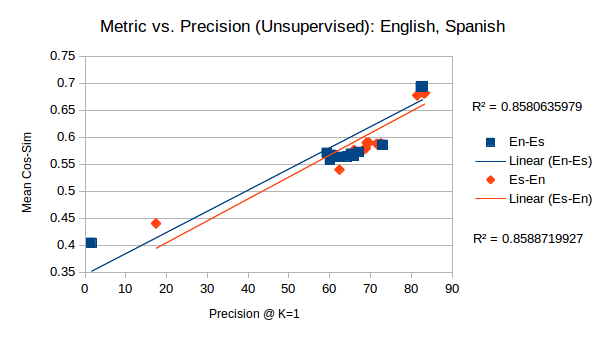
\includegraphics[width=0.6\textwidth]{spanishCorr}
  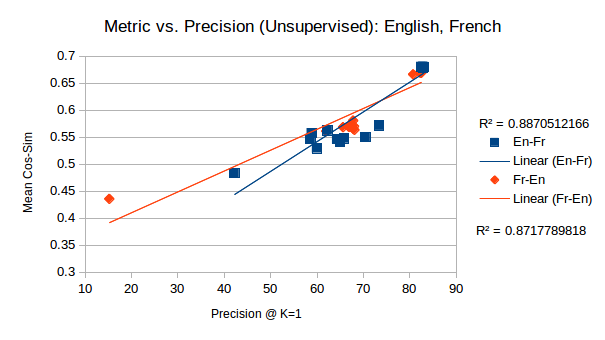
\includegraphics[width=0.6\textwidth]{frenchCorr}
  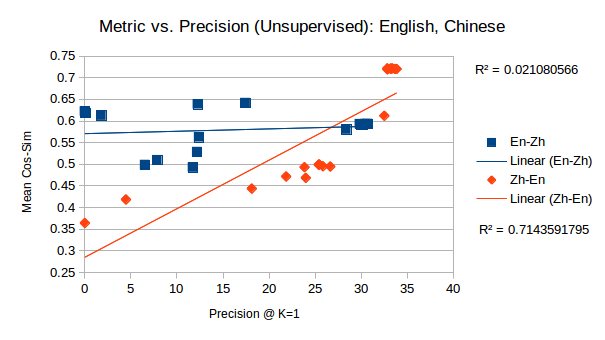
\includegraphics[width=0.6\textwidth]{chineseCorr}
  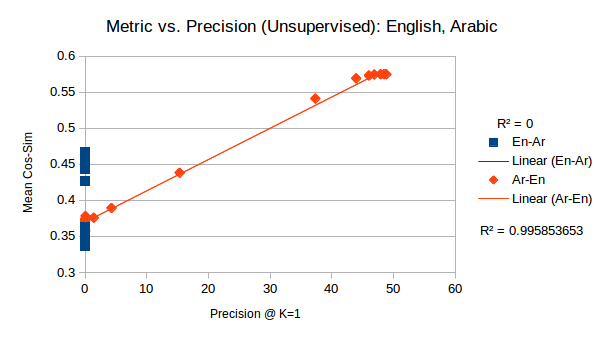
\includegraphics[width=0.6\textwidth]{arabicCorr}
  \caption{Unsupervised CSLS Score vs. Word Translation Precision graphs for 4 language pairs}
\end{figure}

As stated before, if the model validation criterion does not correlate with
precision, there is little chance it will successfully improve. This
explains why language pairs with low correlation also achieve low precision values.

\subsection*{Transliteration}

Due to a lack of compute resources we could perform
only very limited hyperparameter optimization.
All results reported here are from model configurations
with a bidirectional one layer GRU in the encoder,
a one layer GRU in the decoder,
and all RNN cells having 120 units.
We clip gradients to a norm of 5,
apply dropout with rate 0.5 between the encoder and the decoder,
and train with an ADAM optimizer with TensorFlow default hyperparameters
\footnote{https://www.tensorflow.org/api\_docs/python/tf/keras/optimizers/Adam}
We use accuracy on the validation set as an early-stopping metric
with a patience of three epochs.
For decoding we use beam search with ten beams.

\begin{table}[h]
  \centering
  \begin{tabular}{r | c c c c}
    \toprule
    Training Data & Accuracy & MRR@5 & CER* & CER \\
    \midrule
    our pairs & 0.007 & 0.011 & 0.741 & 0.866 \\
    our pairs + CMU & 0.021 & 0.031 & 0.717 & 0.844 \\
    \bottomrule
  \end{tabular}
  \caption{Results of learning transliteration on our generated word
    translations. Evaluated on MUSE data}
  \label{tab:our-muse}
\end{table}

We conducted an experiment to learn transliteration from word translations,
according to the methods section above.
We also conducted an experiment with multitask learning
using our translations for the Japanese script.
As you can see in Table \ref{tab:our-muse},
the model did not succeed in learning transliteration
from the dataset we generated with word translation.
Adding in multitask learning with pronunciation does triple the accuracy,
but even tripled it is still only 2.1\%.

\begin{table}[h]
  \centering
  \begin{tabular}{r | c c c c}
    \toprule
    Training Data & Accuracy & MRR@5 & CER* & CER \\
    \midrule
    eob & 0.403 & 0.486 & 0.240 & 0.312 \\
    eob + CMU & 0.441 & 0.526 & 0.222 & 0.290 \\
    \midrule
    ideal model (memorized MUSE data) & 0.959 & 0.979 & 0.021 & 0.016\\
    \bottomrule
  \end{tabular}
  \caption{Other models evaluated on MUSE data}
  \label{tab:other-muse}
\end{table}

For comparison,
Table \ref{tab:other-muse} contains the results of evaluating
the models trained on other data on the MUSE set.
Since the MUSE data has some ambiguity,
i.e. it provides multiple translations for some words,
We also calculate the ceiling for each metric
that could be reached by memorizing the test data.
We note that that ceiling isn't
the ceiling that could be reached by the ideal transliterator,
as the MUSE data does contain some translations that are not transliterations
(even when filtered to katanaka-English pairs).

\begin{table}[h]
  \centering
  \begin{tabular}{r | c c c c}
    \toprule
    Training Data & Accuracy & MRR@5 & CER* & CER \\
    \midrule
    eob & 0.500 & 0.578 & 0.154 & 0.197 \\
    eob + CMU & 0.535 & 0.614 & 0.147 & 0.189 \\
    \midrule
    ideal model (memorized eob data) & 0.935 & 0.967 & 0.030 & 0.025 \\
    \bottomrule
  \end{tabular}
  \caption{Models evaluated on test split of eob data}
  \label{tab:eob-results}
\end{table}

We conducted a normal training experiment on the eob data,
and one with multitask learning as described in the methods section,
and report the results in Table \ref{tab:eob-results}.
Since the eob data contains multiple transliterations for some words
We also report the ceiling achievable for each metric
by a deterministic transliterator.

\begin{table}[h]
  \centering
  \begin{tabular}{r | c c c c}
    \toprule
    Model & 1 - WER & WER & CER \\
    \midrule{}
    Seq2Seq, bidirectional one layer GRU & 0.454 & 0.546 & .226 \\
    best Seq2Seq model & .498 & .502 & .202 \\
    best of any model & .498 & .502 & .181 \\
    \bottomrule
  \end{tabular}
  \caption{Rosca and Breuel \cite{Rosca2016SequencetosequenceNN} (Google neural
    transliteration paper)}
  \label{tab:baseline-results}
\end{table}

For comparison we reprint excerpted results
from Rosca and Breuel \cite{Rosca2016SequencetosequenceNN}
in Table \ref{tab:baseline-results}.
They are not exactly comparable
because we do not have access to the test split they used.
Furthermore,
they report a word error rate,
but the determination of words when comparing katakana strings
isn't trivial or explained in their paper.
We can try and estimate their accuracy
by one minus the word error rate,
which might be exactly correct if they don't segment katakana strings.
By that estimate our results are in the same ballpark,
indeed our results for learning transliteration
with a Seq2Seq model and no multitask learning
are within a few tenths of a percent of eachother.
That is rather lucky,
as they performed comparatively exhaustive hyperparameter tuning
and used much larger models.
It is possible that the test split we randomly created
is easier than the test split they used.

The 53.5\% accuracy result with multitask learning
is better than any result in the baseline paper,
but a 3.5\% delta seems weak
in the context of larger deltas between other model architectures
that they report results for
(see difference between the bidirectional GRU and the best Seq2Seq).
Furthermore,
if it is the case that their test split was harder
then it may not represent an improvement over what they achieved.
Although not explicitly quantified here
(for lack of time in the home stretch of the project)
our subjective impression,
from running various experiments over the course of the project,
is that using the pronunciation data
did consistently improve the accuracy of the model.

\section*{Conclusions}

While Conneau et al.'s Word Translation Without Parallel Data approach
works well with closely related language pairs, it completely fails
with the English-Japanese pair, along with pairs of comparable distance.
The possible reasoning for this includes noisy pretrained language
embeddings and a domain-adversarial approach that is highly sensitive
to hyperparameters, but we claim that the predominant cause of this
poor performance is the weak correlation between their proposed
validation criterion and actual word translation precision.

Future work in this task may include measuring performance when translating
to an intermediate language first (i.e. Japanese $\rightarrow$ Korean
$\rightarrow$ English), along with improving the validation criterion to
deal with distant language pairs.

A multitask learning approach for utilizing pronunciation information
to improve English to Japanese transliteration
showed promising preliminary results,
but ones that were weak relative to the scale of variation
between various model architectures as reported
in the baseline paper \cite{Rosca2016SequencetosequenceNN}.
The next step to proving the usefulness of our approach
would be to conduct a more thorough study,
varying the model architecture and performing cross-validation
to show that the pronunciation data is consistently helpful.

Another possibility to consider
is changing the way we handle the multiple scripts.
Since we have separate decoders in our approach,
the supervision from the pronunciation data
can only help transliteration by affecting the encoder.
One can easily imagine creating a single decoder
which could output multiple target scripts:
sharing decoders might allow the supervision from pronunciation
to benefit transliteration in both encoding and decoding.

\section*{Individual Tasks}

Derick had full responsibility for the transliteration half of the project.
That included preprocessing our outside data sources,
writing code for the models/training/evaluation,
and running experiments.

Although Derick has worked on some closely related things before,
this project is not part of or an extension of any project
that either author has done before.
It is also not likely that this work will become a part of any future project.

Tim had full responsibility for the word translation without parallel data
half of the project, which included reproducing the results of the paper,
modifying the released codebase to generate translations for the
transliteration half of the project, reproducing the results on the new
language pairs, and the analysis on the correlation between the proposed
metric and word translation precision.

Tim did not have any direct experience in machine translation prior to this
project, although he does have experience with the domain-adversarial
approach used and neural networks.

\bibliography{doc}{}
\bibliographystyle{plain}
\end{document}
%%% Local Variables:
%%% mode: latex
%%% TeX-engine: xetex
%%% TeX-master: t
%%% End:
